\documentclass[11pt]{article}
%Gummi|063|=)
\title{\textbf{Algorithms I -- supervision 6}}
\author{James Wood}
\usepackage{listings}
\usepackage{bold-extra}
\usepackage{xcolor}
\usepackage{amsmath}
\usepackage{enumitem}
\usepackage{tikz}
\usetikzlibrary{arrows}

\lstset{
  basicstyle=\small,
  basewidth=0.5em,
  frame=single,
  breaklines=true,
  %postbreak=\raisebox{0ex}[0ex][0ex]{
  %  \ensuremath{\color{red}\hookrightarrow\space}
  %}
  language=python,
  literate=
    {<=}{{\(\leq\)}}1
    {>=}{{\(\geq\)}}1
    {&&}{{\(\wedge\)}}1
    {||}{{\(\vee\)}}1
    {->}{{\(\rightarrow\)}}1
}

\tikzset{
  treenode/.style = {align=center, inner sep=0pt, text centered,
    font=\sffamily},
  bnode/.style = {treenode, circle, white, draw=black,
    fill=black, text width=1.5em},
  rnode/.style = {treenode, circle, red, draw=red,
    text width=1.5em, very thick},
  leaf/.style = {treenode, rectangle, draw=black,
    minimum width=0.5em, minimum height=0.5em}
}

\begin{document}
\renewcommand{\labelenumi}{(\alph{enumi})}
\renewcommand{\labelenumii}{(\roman{enumii})}

\maketitle

\section{Dijkstra}
\begin{enumerate}
\item The algorithm starts at a given vertex, whose distance is marked as 0. All edges connected to this vertex are added to a priority queue, sorted by weight in ascending order (lightest first). The first vertex in the queue is then traversed, and the new vertex is given a distance equal to the weight of the edge. Its edges are then added to the queue, and the process is repeated (assigning distances equal to the weight of the edge plus the distance given to the vertex at the other end of the edge). Edges between vertices with distances already calculated are removed from the queue. Assuming a connected graph, the algorithm terminates when all vertices have been assigned a distance, or equivalently when the queue is exhausted.
\item
  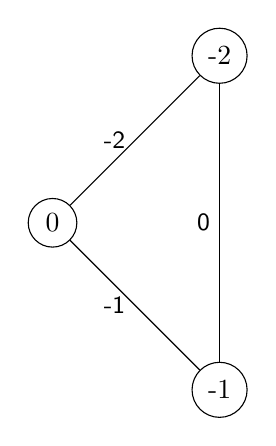
\begin{tikzpicture}[baseline={(1.base)},node distance=3cm,main node/.style={circle,draw}]
    \node[main node] (1) {-2};
    \node[main node] (2) [below left of=1] {0};
    \node[main node] (3) [below right of=2] {-1};

    \path[every node/.style={font=\sffamily\small}]
    (1) edge node [left] {-2} (2)
    (2) edge node [left] {-1} (3)
    (3) edge node [left] {0} (1);
  \end{tikzpicture}
\end{enumerate}

\end{document}